\documentclass[twoside, 11pt]{memoir}
%
% gmverse gives us lines that break on the right with the remainder
% flush right.  It can also be used to centre a verse on the page by
% its optical centre.
\usepackage{gmverse}
%
% Use a sans-serif font designed for continuous text.
\usepackage{helvet}
\renewcommand{\rmdefault}{phv}
% Allow scale factors for dimensions without \dimexpr
\usepackage{calc}
\usepackage{graphicx}
\graphicspath{{./IMAGES}{../IMAGES/}{./}}

% For debugging
% Lipsum generates dummy text
\usepackage{lipsum}

% showframe puts a red frame around text and heading areas
% UNcomment to enable.
%\usepackage{showframe}
%\renewcommand*\ShowFrameColor{\color{red}}

% for debugging: put a tight frame just around the inside of
% something.
% Add around whatever you want to see the boundary of.
\def\tightframe#1{
  \begingroup%
  \fboxrule1pt\fboxsep-1pt%
  \fbox{#1}
  \endgroup
}
% Adjust these to get more debugging oiutput
%\showboxdepth=\maxdimen
%\showboxbreadth=\maxdimen
%\tracingoutput=1
%\tracingonline=1


% Printing on A5 paper
\stockav
% Trim 6mm off outer edge, to make page edges even.
\settrims{0mm}{6mm}
% surprised the class doesn't do this:
\setlength{\paperwidth}{\stockwidth}
\addtolength{\paperwidth}{-\trimedge}
\setlength{\paperheight}{\stockheight}
% spine, fore-edge, ratio
\setlrmarginsandblock{19mm}{10mm}{*}
% allowance for spine -- no need if we're binding in a signature
%\setbinding{5mm}
% upper, lower, ratio
\setulmarginsandblock{25mm}{12mm}{*}
% Make headsep big enough for poem titles.
\setlength{\headsep}{15mm}
% amount of vertical space occupied by header and footer text
\setheadfoot{3ex}{3ex}
% Page height 210mm; text starts 25mm from top, 19mm from spine.
% Page width is 142mm; text width 113mm
% Page number and rule are \headsep (15mm) above the text.
% Poem titles and taglines go under the rule and over the poem.
\checkandfixthelayout[classic]
%
% Calculate where to put titles: move into \headsep space between rule
% and textblock.  Baseline of text moves up...
\newlength{\titledrop}
\titledrop\dimexpr-\headsep-\baselineskip

% we're doing our own stanza spacing.
\setlength{\verseskipbefore}{0pt}
\setlength{\verseskipafter}{0pt}
\setlength{\parindent}{0pt}

% Poem environment
% Full poem starts at the top of a page
% optional first argument is the index term
% other arguments are the poem title and the left margin
% thus \begin{poem}[limerick, A]{A Limerick}{10mm}
\newenvironment{poem}[3][]{%
  % Add first arg to index if it's there;
  % otherwise use second arg.
  \def\indexitem{#1}
  \ifx\indexitem\empty\index{#2}\else\index{#1}\fi%
  % set up the indent
  \verseleftskip#3
  \clearpage % Start at top of page
  % Move heading into heading space
  % titledrop is negative
    \mbox{}\vskip\titledrop
    \vbox to \headsep{\vskip 1ex% move title down from line
    \hbox{\Large\textbf{\MakeUppercase{#2}}}}
}{% At end of poem, leave gap, encourage page break
  \vskip2ex plus \fill\filbreak}

% A tagline is a dedication or other info subordinate to the title.
% It goes in the space between the title and the top of the text
% This means that the top of a multi-page poem will be aligned.
\def\tagline#1{%
  % Move to the same place as the title starts
  \vskip\titledrop
  % Use vtop to overlap what's there
  \vtop to \headsep{%
    \vskip1.6\baselineskip% skip over title
    \hbox to \textwidth{\hskip\verseleftskip\textsl{#1}\hfil}%
  }%
}

% A micropoem is a short poem, styled to fit on a page not at the top.
% Same arguments as fro the poem environment.
\newenvironment{micropoem}[3][]{%
  \ifx\newenvironment#1\newenvironment\index{#2}\else\index{#1}\fi
  \verseleftskip#3
  \setlength{\partopsep}{0pt}
  \leavevmode
  \mbox{}\vskip2ex plus \fill%
  \vbox to 0.5\headsep{%
    \vfil%
    \hbox to \textwidth{%
      \hspace{#3}\Large\textbf{\MakeUppercase{#2}}\hfil%
    }%
    \vfil
  }
  \normalsize
}{\vskip4ex}

% A cmicropoem is a micropoem centred on the page.
% Usually it'll use the cstanza environment for stanzas.
\newenvironment{cmicropoem}[3][]{%
  \ifx\newenvironment#1\newenvironment\index{#2}\else\index{#1}\fi
  \verseleftskip#3
  \setlength{\partopsep}{0pt}
  \mbox{}\vskip 2ex plus \fill%
  \vbox to 0.5\headsep{%
    \vfil
    \hbox to \textwidth{%
      \mbox{}\hfil\Large\textbf{\MakeUppercase{#2}}\hfil
    }%
    \vfil
  }
  \normalsize
}{\vskip4ex}

% A stanza is a section of poetry.
\newenvironment{stanza}%
{\verse}{\endverse\vskip 10pt\filbreak}

% A cstanza i a centred stanza
\newenvironment{cstanza}%
{\parskip0pt\par\centering}{\vskip10pt\filbreak}

% An altstanza is a stanza with a different indentation from the
% stanzas around it.  Indentation is given by the (optional) argument;
% if not given, it's 1.3 times the left skip given to the surrounding
% poem environment.
\newenvironment{altstanza}[1][1.3\verseleftskip]%
{\verseleftskip#1\verse}{\endverse\vskip 10pt\filbreak}

% A wide stanza is one that is too wide to lookgood with the standard
% settings.
% Its argument is the longest line in it, or its fellow stanzas.
% It will be optically centred on that line's width.
% In a poem with more than one wide stanzas, that line should be the
% same for all widestanzas
\newenvironment{widestanza}[1]{%
  \begingroup\versemaxline{#1}\verseleftskip=0mm\verse%
}%
{\endverse\vskip10pt\endgroup\filbreak}

% Set headers and footers.
\ifdraftdoc\makeoddfoot{Ruled}{\today}{DRAFT}{}
\makeevenfoot{Ruled}{}{DRAFT}{\today}
\else
\makeoddfoot{Ruled}{}{}{}
\makeevenfoot{Ruled}{}{}{}
\fi
\makeevenhead{Ruled}{\thepage}{}{}
\makeoddhead{Ruled}{}{}{\thepage}


% We want an index
\makeindex
% Make the index look like everything else.
% It's probably possible to do this by fiddling with the (many)
% parameters for 'chapter', but it's easier just to redefine the
% index environment.

\makeatletter
\renewenvironment{theindex}{
  \clearpage
  \mbox{}\vskip\titledrop
  \vbox to \headsep{\vskip 1ex% move title down from line
    \hbox{\LARGE\textbf{Index}}}
  \parskip\z@ \@plus .3\p@\relax
  \let\item\@idxitem}{}
\makeatother

% More debugging
%\typeout{\noexpand\topskip = \the\topskip}
%\typeout{\noexpand\baselineskip = \the\baselineskip}
%\typeout{\noexpand\headsep = \the\headsep}
% paperwidth is 148mm - trim 6mm = 142mm.
% spinemargin is 18mm
% upper margin is 25mm
% right margin is 10mm
% lower margin is 10mm

% Create cover page; optional argument non-empty
% for verso pages.
\newcommand{\coverpage}[2][]{
  \begingroup
  \def\side{#1}%
  \hbox to \paperwidth{%
    \hbadness=10000%suppress underfull hbox msgs
    \hfuzz=\maxdimen
    \vbox to 0pt{%
      % Move up
      \vskip\dimexpr9mm-\uppermargin\relax%
      % And toward the spine
      \ifx#1\empty\mbox{}\hskip10mm-\spinemargin\relax%
      \else\mbox{}\hskip\dimexpr-4mm\relax\fi%
      % Outer marginal box
      \fbox{% This will warn of overful box because it extends into the margins
        \begin{minipage}{122mm}
          \vbox to 184mm{%
          \hbadness=10000%suppress underfull hbox msgs
            #2%
          }%
        \end{minipage}%
      }%
    }
  }
  \endgroup
}

\begin{document}
\def\theauthor{The Author}
\def\thetitle{TITLE}
\def\thenumber{Volume 4}

\thispagestyle{empty}
\setlength\fboxrule{1mm}
\newsavebox{\titlepage}
\sbox{\titlepage}{%
  \hbadness=10000
  \coverpage{
    \hfuzz=\maxdimen
    \begin{center}
      \vskip22mm
      \fontsize{18mm}{23mm}\selectfont%
      \textsl{\textbf{\thetitle}}\\[5mm]
%
      \fbox{%
        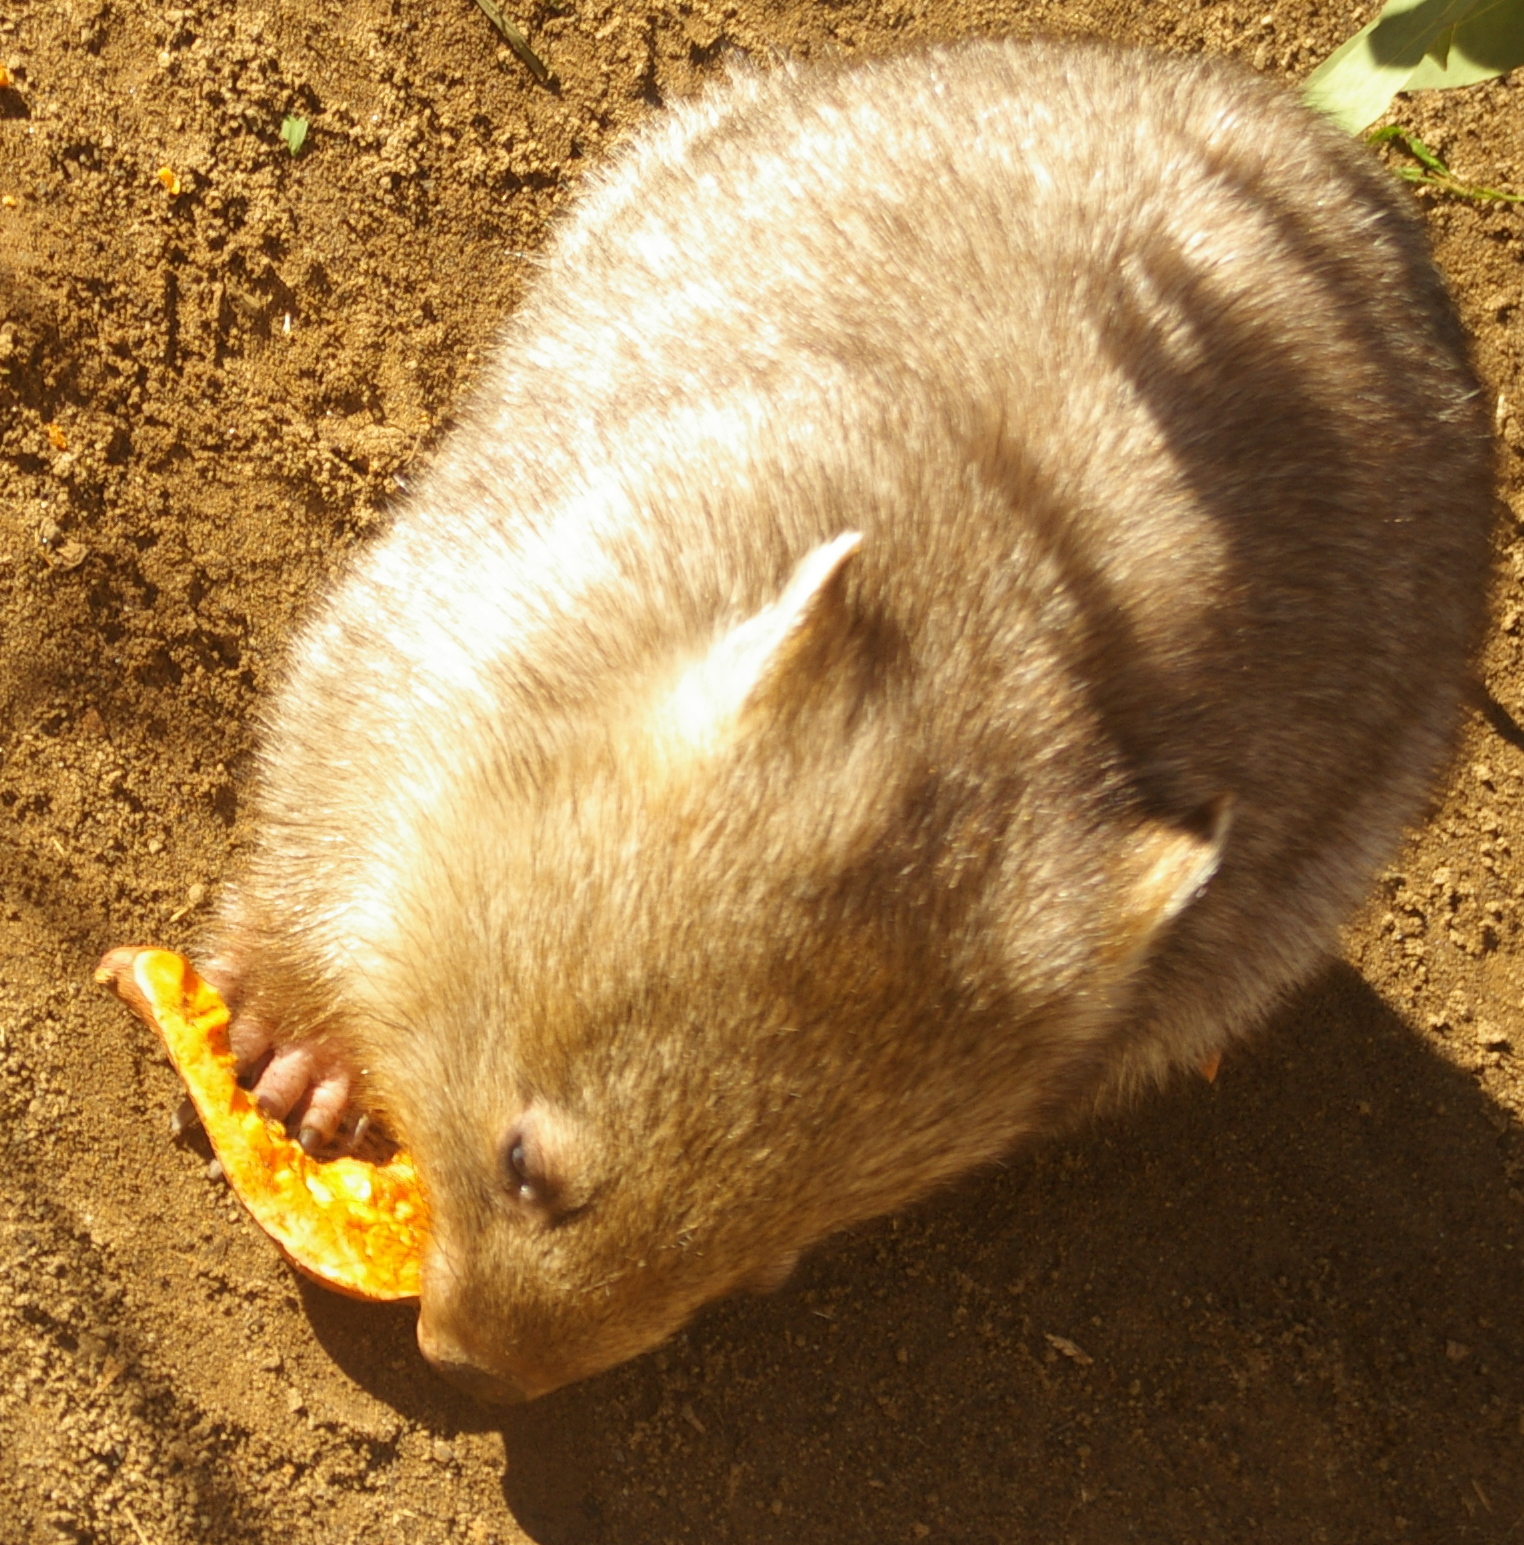
\includegraphics[width=55mm]{baby-wombat
        }%
      }\\
      {\fontsize{6mm}{7mm}\selectfont%
        \textbf{Poetry}}\\
      \Large%
      \textbf{by}\\
      \textbf{\theauthor}\\[15mm]
    \end{center}
    \hfill\textbf{\thenumber}
  }
}

\usebox{\titlepage}
\hfuzz=\maxdimen

\cleartorecto
\thispagestyle{empty}
\usebox{\titlepage}

\setcounter{page}{1}
\cleartoverso
\renewcommand{\thepage}{\roman{page}}
\mbox{}
\begingroup
\normalsize\setlength{\parskip}{0.5ex plus 0.3ex}
 \textbf{NOTES}
  
\endgroup
\vspace*{\fill}
\mbox{}\par
{\small
Copyright \copyright\ 2023 \theauthor\\
All rights reserved.\\
No part of this publication may be reproduced or transmitted, in any
form or by any means, electronic or mechanical, including photocopy,
recording or any information storage and retrieval system, without
permission in writing from the copyright holders.

\begin{center}
ISBN: 123--456--789--0\
\end{center}

}
\vspace*{1cm}
\cleartorecto
\pagestyle{Ruled}
\begingroup
%\myindex{Forward}
\setlength{\parindent}{2em}
{
\centering
\textit{\large Dedication goes here\\}
}
\section*{Foreword}
\lipsum[3-4]

%%% Local Variables:
%%% mode: latex
%%% TeX-master: book.tex
%%% End:

\endgroup
\cleartorecto
\mainmatter

%%% Local Variables:
%%% mode: latex
%%% TeX-master: "why"
%%% End:

\begin{poem}{At the round earth's imagin'd corners}{15mm}
  \tagline{by John Donne}
  \begin{stanza}
    At the round earth's imagin'd corners, blow
Your trumpets, angels, and arise, arise
From death, you numberless infinities
Of souls, and to your scatter'd bodies go;
All whom the flood did, and fire shall o'erthrow,
All whom war, dearth, age, agues, tyrannies,
Despair, law, chance hath slain, and you whose eyes
Shall behold God and never taste death's woe.
But let them sleep, Lord, and me mourn a space,
For if above all these my sins abound,
'Tis late to ask abundance of thy grace
When we are there; here on this lowly ground
Teach me how to repent; for that's as good
As if thou'hadst seal'd my pardon with thy blood.
\end{stanza}
\end{poem}
%%% Local Variables:
%%% mode: latex
%%% TeX-master: "book"
%%% End:

\printindex
% \mbox{}\vskip\titledrop
% \vbox to \headsep{\vskip 1ex% move title down from line
% \hbox{\Large\textbf{\MakeUppercase{Afterthoughts}}}}

%%% Local Variables:
%%% mode: latex
%%% TeX-master: "book"
%%% End:

% Put colophon on inside of back cover.
\newcount\sheetnum
\sheetnum\thesheetsequence
\divide\sheetnum by2\relax%
\typeout{\thesheetsequence `thesheet \the\sheetnum}
\pagestyle{empty}
\mbox{}\ifodd\sheetnum\relax\else\newpage\mbox{}\newpage\mbox{}\fi
\cleartorecto
\vskip\titledrop
\vbox to 0.8\paperheight{
  \vss
  \centering
  Typeset by Peter Chubb in 11pt Helvetica using \LaTeX\ and the
  Memoir document class.
  \vss
}
\clearpage
% back cover.
\thispagestyle{empty}
\setlength\fboxrule{1mm}
\coverpage[verso]{%
  \begin{centering}
    \mbox{}\\[1cm]
    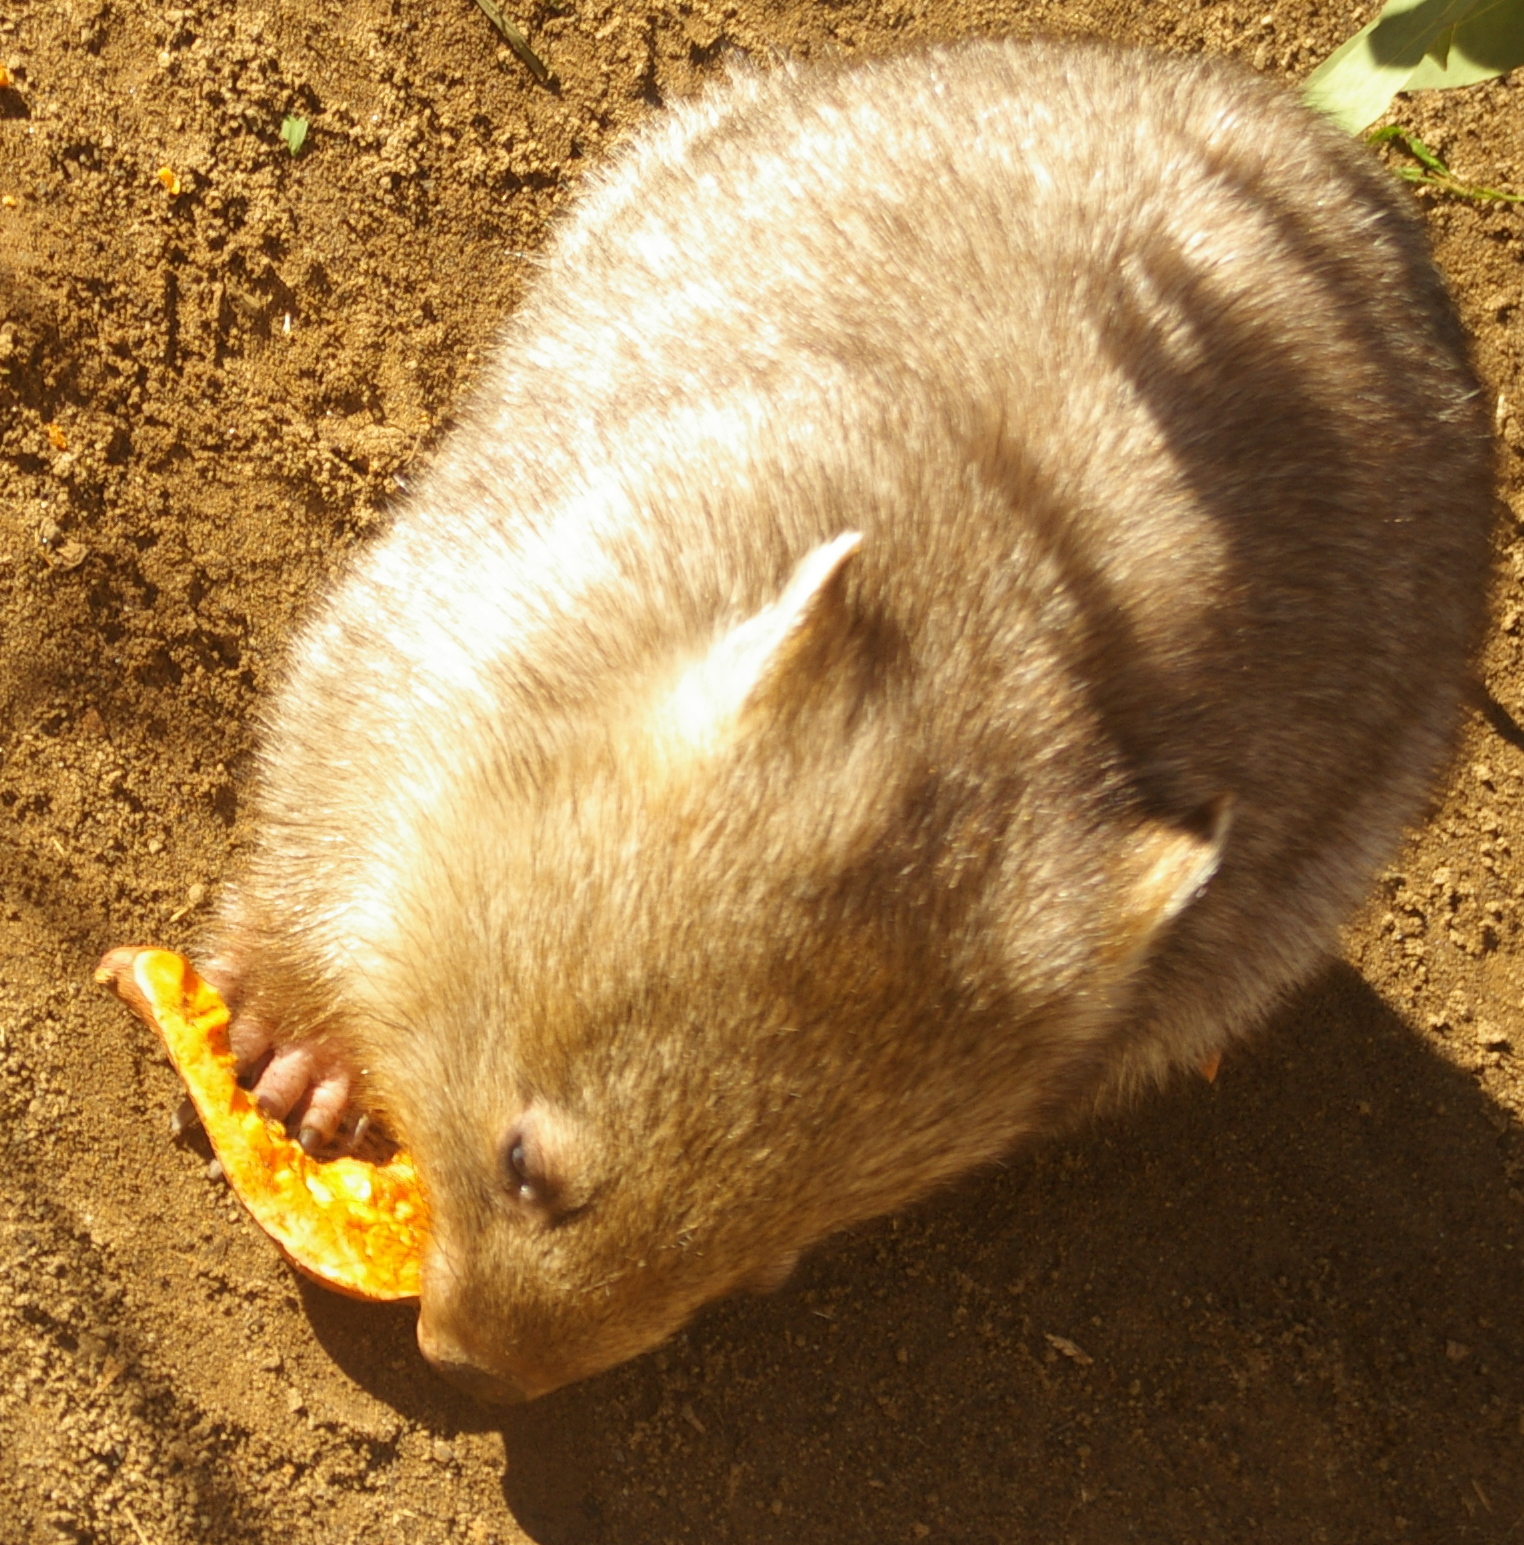
\includegraphics[width=0.8\linewidth]{baby-wombat}\\[5ex]
    \begin{minipage}[h]{0.9\linewidth}
      \textbf{about the author:}
      \lipsum[][1-3]
      \vskip20mm

      \textbf{about the book:}
      \lipsum[2][1-3]

    \end{minipage}\\
  \end{centering}
}

%%% Local Variables:
%%% mode: latex
%%% TeX-master: "book"
%%% End:

\end{document}

%%% Local Variables:
%%% mode: latex
%%% TeX-master: t
%%% End:

